% Created 2019-02-18 Mon 00:04
\documentclass[11pt]{article}
\usepackage[utf8]{inputenc}
\usepackage[T1]{fontenc}
\usepackage{fixltx2e}
\usepackage{graphicx}
\usepackage{longtable}
\usepackage{float}
\usepackage{wrapfig}
\usepackage{rotating}
\usepackage[normalem]{ulem}
\usepackage{amsmath}
\usepackage{textcomp}
\usepackage{marvosym}
\usepackage{wasysym}
\usepackage{amssymb}
\usepackage{hyperref}
\tolerance=1000
\usepackage{minted}
\usepackage{amsthm}
\usepackage[margin=1.0in]{geometry}
\setlength{\parindent}{0pt}
\setlength{\parskip}{\baselineskip}
\author{Thomas Alford}
\date{\today}
\title{Ph21 Problem Set 3}
\hypersetup{
  pdfkeywords={},
  pdfsubject={},
  pdfcreator={Emacs 25.2.1 (Org mode 8.2.10)}}
\begin{document}

\maketitle
\section*{1}
\label{sec-1}
\subsection*{Imports}
\label{sec-1-1}
\begin{minted}[frame=lines,fontsize=\scriptsize]{python}
import numpy as np
import matplotlib.pyplot as plt
from matplotlib.pyplot import imshow
%matplotlib inline
from PIL import Image, ImageFilter
from scipy import ndimage
from scipy.ndimage import filters
\end{minted}

\subsection*{Import an Image}
\label{sec-1-2}

\begin{minted}[frame=lines,fontsize=\scriptsize]{python}
def open_image(fname, print_info=True):
    im  = Image.open(fname)
    if (print_info):
        print('Image format = %s, Image size = %s, Image mode = %s'%(
            im.format, im.size, im.mode))
    return im

def display_image(im):
    imshow(np.asarray(im))
\end{minted}


Let's try importing an image I downloaded earlier:

\begin{minted}[frame=lines,fontsize=\scriptsize]{python}
im = open_image('/Users/tommyalford/Desktop/EdgeDetectImage.jpg')
\end{minted}

\begin{verbatim}
Image format = JPEG, Image size = (2400, 1600), Image mode = RGB
\end{verbatim}

\section*{2}
\label{sec-2}
\subsection*{Disply an Image}
\label{sec-2-1}

We can display it inline with matplotlib:

\begin{minted}[frame=lines,fontsize=\scriptsize]{python}
display_image(im)
\end{minted}

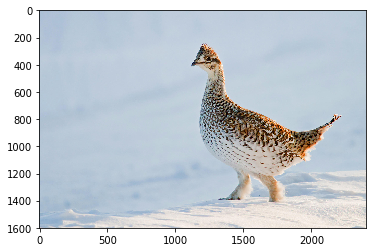
\includegraphics[width=.9\linewidth]{./obipy-resources/333kTu.png}

\section*{3}
\label{sec-3}
Here I would guess that edge detection has something to do with checking the
change in pixel level across different areas and finding where the change is
the largest (if we consider the pixels as datapoints in a multi-variable
function). I'll look on wikipedia for the official way to do it to save time.

Let's see what the existing image filter does:

\subsection*{Official Edge Detection}
\label{sec-3-1}

\begin{minted}[frame=lines,fontsize=\scriptsize]{python}
def get_existing_edge_detection(im):
    edge_im = im.filter(ImageFilter.FIND_EDGES)
    return edge_im
\end{minted}


\begin{minted}[frame=lines,fontsize=\scriptsize]{python}
edge_im = get_existing_edge_detection(im)
plt.imshow(np.array(edge_im), cmap='gray')
plt.show()
\end{minted}

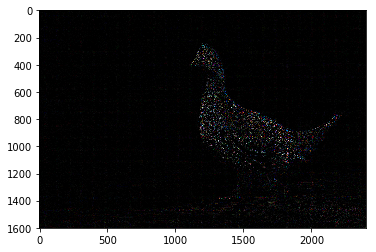
\includegraphics[width=.9\linewidth]{./obipy-resources/333xd0.png}

Looks like it worked pretty well! 

\section*{4}
\label{sec-4}
\subsection*{Blurring}
\label{sec-4-1}

\begin{minted}[frame=lines,fontsize=\scriptsize]{python}
blurred = im.filter(ImageFilter.GaussianBlur(radius=5))
display_image(blurred)
\end{minted}
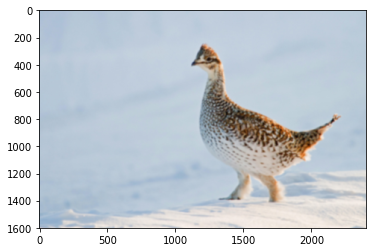
\includegraphics[width=.9\linewidth]{./obipy-resources/333jnD.png}

Here we do see the image as blurry but still visible now. This does seem like
this would be easier for edge detection. We can test with different radaii
later to see which gives us the best edge detection. 5 is probably a little
large.

\section*{5}
\label{sec-5}

\subsection*{Canny Edge Detectionn}
\label{sec-5-1}

Steps:
\begin{itemize}
\item Smooth the image with a Gaussian blurring filter
\item Compute the x and y derivatives at each pixel
\item Take out any pixels which are not local maxima
\item Apply the double threshold to see wich edge pixels are not as 'intense' as
others
\item Get rid of the weak edge pixels which do not share a neighbor with any strong
edge pixels
\end{itemize}

\subsubsection*{Compute X and Y Derivatives}
\label{sec-5-1-1}

\begin{minted}[frame=lines,fontsize=\scriptsize]{python}
def compute_ndimage_grad(im, sigma=1):
    Gx = np.zeros(im.shape);
    Gy = np.zeros(im.shape);
    # use first derivative of a Gaussian
    # x derv
    filters.gaussian_filter(im, sigma=sigma, order=[1, 0], output=Gx,
                            mode='nearest')
    # y derv
    filters.gaussian_filter(im, sigma=sigma, order=[0, 1], output=Gx,
                            mode='nearest')
    magnitude = np.sqrt(Gx**2 + Gy**2)
    direc = np.arctan2(Gy, Gx)
    return magnitude, direc
\end{minted}


\begin{minted}[frame=lines,fontsize=\scriptsize]{python}
blurred = im.filter(ImageFilter.GaussianBlur(radius=3))
gray_blurred = np.array(blurred.convert('L'))
mag, direc = compute_ndimage_grad(gray_blurred)
\end{minted}


\begin{minted}[frame=lines,fontsize=\scriptsize]{python}
plt.imshow(mag, cmap='gray')
plt.show()
\end{minted}

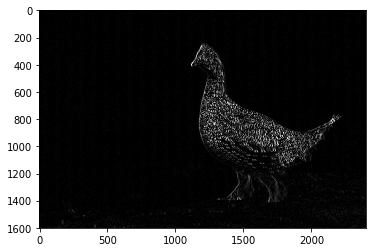
\includegraphics[width=.9\linewidth]{./obipy-resources/33308Z.png}

\subsubsection*{Round Angles}
\label{sec-5-1-2}

Now we need to round direc to the nearest quadrant:

\begin{minted}[frame=lines,fontsize=\scriptsize]{python}
def round_angle(theta):
    # divide by pi/4, round to nearest int (mod 4), muliply by pi/4
    return (np.round(theta / (np.pi / 4)) % 4) * (np.pi / 4)

rounded_direcs = round_angle(direc)
\end{minted}

\subsubsection*{Apply Non-Max Suppression}
\label{sec-5-1-3}

Now we need to apply nonmax suppression to take out any pixel which are not
local maxima:

Pseudocode here:

for each pixel:
\begin{itemize}
\item find neighbors in direction from directional grad
\item if val is larger than neighbor vals, make that an 'edge' in new 'edge array'
\end{itemize}

This will give us our edge pixels. Now we just need to threshhold these values
in some way (keep the mags in the edge array), and then check each neighboring
'blob' of 8 pixels. If the blob has no strong pixels then throw out the weak
pixel.

\begin{minted}[frame=lines,fontsize=\scriptsize]{python}
def get_pixel_diffs(theta):
    # returns the x and y indeces (can be i, i + 1, j, j + 1)
    # theta is already rounded
    # so using sine and cosine and rounding should get us what we want
    return np.array([np.round(np.cos(theta)), np.round(np.sin(theta))])
\end{minted}


\begin{minted}[frame=lines,fontsize=\scriptsize]{python}
def get_ind(r_direcs):
    indices = np.dstack(np.indices(r_direcs.shape))
    diffs = get_pixel_diffs(r_direcs)
    xy_ind = []
    for i, d in enumerate([diffs, -1 * diffs]):
        xind = np.array(indices[:, :, 0] + d[0], dtype='int')
        yind = np.array(indices[:, :, 1] + d[1], dtype='int')
        xy_ind.append([xind, yind])
        
    return xy_ind[0], xy_ind[1]
\end{minted}


\begin{minted}[frame=lines,fontsize=\scriptsize]{python}
def suppress_nonmax(mag, direcs):
    #rounded_direcs = round_angle(direcs)
    pad = np.pad(mag, pad_width=1, mode='constant', constant_values=0)
    # get new indeces from the angles of which we get our neighbors
    pos_ind, neg_ind = get_ind(direcs)
    # get negative neighbors
    neg_slice = pad[neg_ind[0] + 1, neg_ind[1] + 1]
    # get positive neighbors
    pos_slice = pad[pos_ind[0] + 1, pos_ind[1] + 1]
    # now just take max of pos and neg ind slices
    max_vals = np.maximum(neg_slice, pos_slice)
    suppressed_mags = (mag >= max_vals) * mag
    return suppressed_mags
\end{minted}



\begin{minted}[frame=lines,fontsize=\scriptsize]{python}
suppressed_grad = suppress_nonmax(mag, rounded_direcs)
plt.imshow(suppressed_grad, cmap='gray')
\end{minted}

\begin{verbatim}
<matplotlib.image.AxesImage at 0x161d0af28>
\end{verbatim}
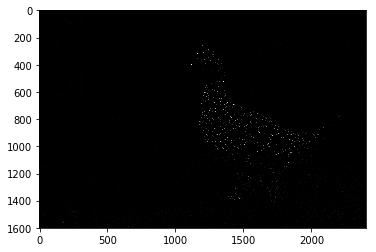
\includegraphics[width=.9\linewidth]{./obipy-resources/333BHg.png}

This looks pretty close to the earlier edge detection image now! All we have to
do is double threshhold the pixels now to remove any weak gradient values

\subsubsection*{Double Threshold}
\label{sec-5-1-4}

\begin{minted}[frame=lines,fontsize=\scriptsize]{python}
plt.hist(suppressed_grad[suppressed_grad > 0], bins=100)
plt.xlabel('intensity')
plt.ylabel('counts')
plt.xlim([0, 5])
plt.show()
\end{minted}

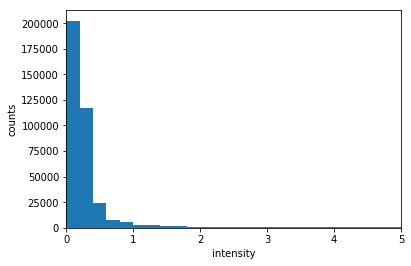
\includegraphics[width=.9\linewidth]{./obipy-resources/333ORm.png}

Looking at the histogram of gradient values, we'll try thresholding for a low
value of .5 and a high value of 3.

\subsubsection*{Applying Hysteresis}
\label{sec-5-1-5}
\begin{minted}[frame=lines,fontsize=\scriptsize]{python}
def get_8_neighbors(mag):
    indices = np.dstack(np.indices(mag.shape))
    # these diffs are basically (1, 0), (1, 1), (0, 1), (1, -1), (0, -1), ...
    diffs = [(0, 1), (1, 0), (0, -1), (-1, 0), (1, 1), 
             (1, -1), (-1, 1), (-1, -1)]
    xy_ind = []
    for d in diffs:
        xind = np.array(indices[:, :, 0] + d[0], dtype='int')
        yind = np.array(indices[:, :, 1] + d[1], dtype='int')
        xy_ind.append([xind, yind])
        
    return xy_ind
def apply_hysteresis(low_thresh, high_thresh, grad): 
    pad = np.pad(grad, pad_width=1, mode='constant', constant_values=0)
    # get new indeces from the angles of which we get our neighbors
    neighbor_inds = get_8_neighbors(grad)
    slices = []
    for ind in neighbor_inds:
        ind_slice = pad[ind[0] + 1, ind[1] + 1]
        slices.append(ind_slice)
    # if we get the max value of all the slices, and this value is below the 
    # strong threshold cutoff, we know that we can remove the weak pixel
    max_intensity = np.amax(np.array(slices), axis=0)
    hyster_mask = ((max_intensity < high_thresh) & (grad < low_thresh))
    # this shows any values which should be suppressed
    # so we need to invert this before masking
    return grad * np.logical_not(hyster_mask)
\end{minted}


Here we'll also put all edge pixels at the maximum brightness in order to see
them more clearly:

\begin{minted}[frame=lines,fontsize=\scriptsize]{python}
hyster_edge = apply_hysteresis(1, 3, suppressed_grad)
# make all edges very bright now to easily see them
max_vals = 255 * (hyster_edge > 0)
plt.imshow(max_vals, cmap='gray')
plt.show()
\end{minted}

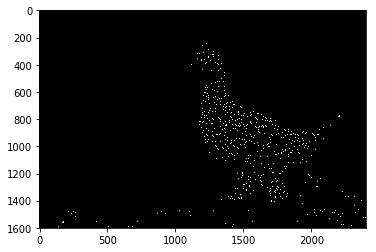
\includegraphics[width=.9\linewidth]{./obipy-resources/333n5H.png}

Looks pretty good!

\section*{Optimization}
\label{sec-6}
\subsection*{Try over various filter, images}
\label{sec-6-1}

Let's put this all into one method now:

\begin{minted}[frame=lines,fontsize=\scriptsize]{python}
def get_edge_detection(im, gaussian_r, low_thresh, high_thresh,
                       stencil_width=1, apply_max=True):
    blurred = im.filter(ImageFilter.GaussianBlur(radius=gaussian_r))
    gray_blurred = np.array(blurred.convert('L'))
    mag, direc = compute_ndimage_grad(gray_blurred, sigma=stencil_width)
    rounded_direcs = round_angle(direc)
    suppressed_grad = suppress_nonmax(mag, rounded_direcs)
    hyster_edge = apply_hysteresis(low_thresh, high_thresh, suppressed_grad)
    max_vals = 255 * (hyster_edge > 0)
    if (apply_max):
        return max_vals
    return hyster_edge
\end{minted}


Now we can try this over different radaii and thresholds for our initial
blurring filter:

\begin{minted}[frame=lines,fontsize=\scriptsize]{python}
plt.imshow(get_edge_detection(im, 2, 1, 3, stencil_width=.4, apply_max=True),
           cmap='gray')
\end{minted}

\begin{verbatim}
<matplotlib.image.AxesImage at 0x17115ac88>
\end{verbatim}
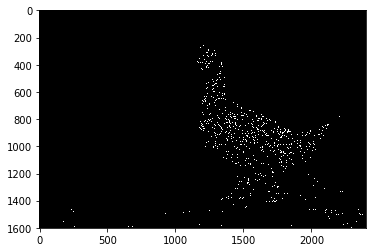
\includegraphics[width=.9\linewidth]{./obipy-resources/333DQi.png}

Let's compare this now to using the original image and then using PIL's edge
detection: we'll also apply some hysteresis and make each pixel the maximum
intensity to better see these edges.

\begin{minted}[frame=lines,fontsize=\scriptsize]{python}
blurred_im = im.filter(ImageFilter.GaussianBlur(radius=0))
gray_blurred_im = blurred_im.convert('L')
edge_im = np.array(get_existing_edge_detection(gray_blurred_im))
hyster_edge = apply_hysteresis(20, 50, edge_im)
max_vals = 255 * (hyster_edge > 0)
plt.imshow(max_vals, cmap='gray')
\end{minted}

\begin{verbatim}
<matplotlib.image.AxesImage at 0x137329550>
\end{verbatim}
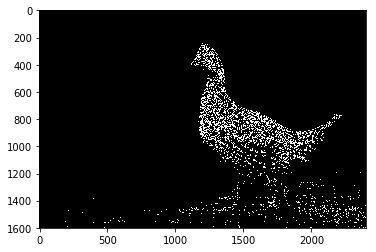
\includegraphics[width=.9\linewidth]{./obipy-resources/333cjn.png}

\subsubsection*{Additional Images}
\label{sec-6-1-1}

We'll look at a couple more images now. Note: I'm only including the final
choices for thresholds and blur radaii for our own filter in order to keep
things at a reasonable length. There was a decent amount of trial-and-error in
order to correctly find the items we wanted.

\begin{minted}[frame=lines,fontsize=\scriptsize]{python}
def plot_comparisons(im, blur_r, low, high, PIL_low, PIL_high, stencil_width=1,
                     apply_max=True):
    fig, axes = plt.subplots(2, 2, figsize=(8, 8))
    axes[0][0].imshow(np.asarray(im))
    axes[0][0].set_title('Original Image')
    blurred = im.filter(ImageFilter.GaussianBlur(radius=blur_r))
    axes[1][0].imshow(blurred, cmap='gray', label='blurred image')
    axes[1][0].set_title('Blurred Image')
    axes[0][1].imshow(get_edge_detection(
        im, blur_r, low, high, stencil_width=stencil_width,
        apply_max=apply_max), cmap='gray')
    axes[0][1].set_title('Own Canny Edge Detector')
    gray_blurred_im = im.convert('L')
    edge_im = np.array(get_existing_edge_detection(gray_blurred_im))
    hyster_edge = apply_hysteresis(PIL_low, PIL_high, edge_im)
    max_vals = 255 * (hyster_edge > 0)
    if (apply_max):
        axes[1][1].imshow(max_vals, cmap='gray')
    else:
        axes[1][1].imshow(edge_im, cmap='gray')
    axes[1][1].set_title('PIL Edge Detector')
\end{minted}


\begin{minted}[frame=lines,fontsize=\scriptsize]{python}
meme2 = open_image('/Users/tommyalford/Desktop/meme2.jpg', print_info=False)
plot_comparisons(meme2, 1, 3, 200, 30, 200, stencil_width=1, apply_max=True)
\end{minted}

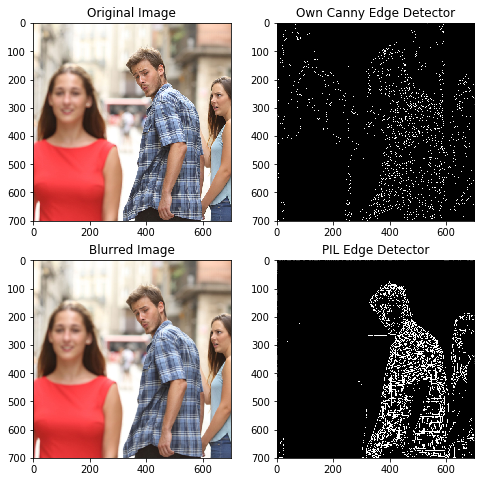
\includegraphics[width=.9\linewidth]{./obipy-resources/333nyT.png}

Here PIL's image does look much crisper, but it's also completely missing the
girl on the left..


\begin{minted}[frame=lines,fontsize=\scriptsize]{python}
velvet = open_image('/Users/tommyalford/Desktop/velvet.jpg', print_info=False)
plot_comparisons(velvet, 0, 3, 20, 50, 250, stencil_width=1, apply_max=True)
\end{minted}

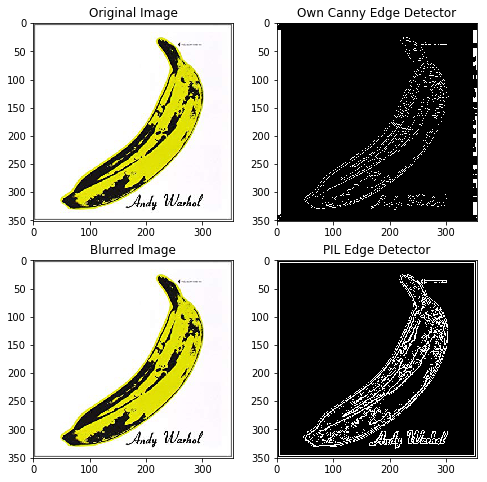
\includegraphics[width=.9\linewidth]{./obipy-resources/333NeH.png}

This image was probably a lot easier to edge detect on, and both detectors
worked pretty well. The PIL detector actually has the writing as readable,
whereas our edge detector didn't get the writing too clearly. Attempts to make
this work without blurring the image didn't result in any better results at
readable writing, and the banana edge detection was worse as well.

\subsection*{Conclusion}
\label{sec-6-2}
After completing this assigment, my thoughts on edge detectors begin to mirror
my thoughts from the start of the assignment: what is an edge? It seems like
edge detectors don't even really know themselves until you tell them what you
want them to look for. Even PIL's filter generally needed some thresholding to
get rid of some of really low-intensity 'edges' it still had in its
images. However, regardless it is pretty magical what a simple stencil can do
do suppress everything besides the edges in an image. The nonmax suppression
and thresholding parts are also nice, but the real bulk of the algorithm seems
to be done purely with the gradient.
% Emacs 25.2.1 (Org mode 8.2.10)
\end{document}
